% answers.tex —— 2002 年·全国新课程卷·理科 · 参考答案与详细解析片段
% 由 tools/generate_projects.py 依来源总账自 2002/2002_数学真题_全国新课程理_试题.md + 2002/2002_数学真题_全国新课程理_解析正文.md + 2002/2002_数学真题_全国新课程理_答案要点.md 生成，勿手改（改源 MD 后重跑）


\begin{gktip}
固定源 PDF 为印刷页码 114–115 的两页题面，不附答案。以下解析均依据题面独立复算；第 18 题图形在 LaTeX 工程中以 TikZ/PGFPlots 矢量图重绘。
\end{gktip}

\gkpart{一、选择题}

\begin{answer}
\gksolhead{1}{}

\textbf{题目}：

\Needspace{5\baselineskip}
曲线

\nopagebreak[4]
\[
\begin{cases}
x=\cos\theta,\\
y=\sin\theta
\end{cases}
\qquad(\theta\text{ \text{为参数}})
\]

上的点到两坐标轴的距离之和的最大值是\mbox{（　　）}

（A）$\dfrac12$　　（B）$\dfrac{\sqrt2}{2}$　　（C）$1$　　（D）$\sqrt2$

\Needspace{4\baselineskip}
\textbf{解析}

\Needspace{5\baselineskip}
曲线上的点为单位圆上的点，点 $(\cos\theta,\sin\theta)$ 到两坐标轴的距离之和为

\nopagebreak[4]
\[
|\cos\theta|+|\sin\theta|
\leqslant\sqrt{2(\cos^2\theta+\sin^2\theta)}
=\sqrt2.
\]

等号在 $|\cos\theta|=|\sin\theta|$ 时取得，最大值为 $\sqrt2$。

\gkanswer{答案：D}

\end{answer}
\begin{answer}
\gksolhead{2}{}

\textbf{题目}：

\Needspace{5\baselineskip}
复数

\nopagebreak[4]
\[
\left(\frac12+\frac{\sqrt3}{2}i\right)^3
\]

的值是\mbox{（　　）}

（A）$-i$　　（B）$i$　　（C）$-1$　　（D）$1$

\Needspace{4\baselineskip}
\textbf{解析}

\Needspace{5\baselineskip}
由

\nopagebreak[4]
\[
\frac12+\frac{\sqrt3}{2}i=\cos\frac\pi3+i\sin\frac\pi3,
\]

\Needspace{5\baselineskip}
故

\nopagebreak[4]
\[
\left(\frac12+\frac{\sqrt3}{2}i\right)^3
=\cos\pi+i\sin\pi=-1.
\]

\gkanswer{答案：C}

\end{answer}
\begin{answer}
\gksolhead{3}{}

\textbf{题目}：

已知 $m\text{、}n$ 为异面直线，$m\subset$ 平面 $\alpha$，$n\subset$ 平面 $\beta$，$\alpha\cap\beta=l$，则 $l$\mbox{（　　）}

（A）与 $m\text{、}n$ 都相交

（B）与 $m\text{、}n$ 中至少一条相交

（C）与 $m\text{、}n$ 都不相交

（D）至多与 $m\text{、}n$ 中的一条相交

\Needspace{4\baselineskip}
\textbf{解析}

若 $l$ 既不与 $m$ 相交，也不与 $n$ 相交，则 $m\parallel l$ 且 $n\parallel l$，从而 $m\parallel n$，与异面直线矛盾。因此 $l$ 至少与 $m\text{、}n$ 中的一条相交。

\gkanswer{答案：B}

\end{answer}
\begin{answer}
\gksolhead{4}{}

\textbf{题目}：

不等式 $(1+x)(1-|x|)>0$ 的解集是\mbox{（　　）}

（A）$\{x\mid 0\leqslant x<1\}$

（B）$\{x\mid x<0\text{ \text{且} }x\neq-1\}$

（C）$\{x\mid -1<x<1\}$

（D）$\{x\mid x<1\text{ \text{且} }x\neq-1\}$

\Needspace{4\baselineskip}
\textbf{解析}

当 $x\geqslant0$ 时解为 $0\leqslant x<1$；当 $x<0$ 时解为 $x<0$ 且 $x\neq-1$。合并得 $x<1$ 且 $x\neq-1$。

\gkanswer{答案：D}

\end{answer}
\begin{answer}
\gksolhead{5}{}

\textbf{题目}：

在 $(0,2\pi)$ 内，使 $\sin x>\cos x$ 成立的 $x$ 的取值范围是\mbox{（　　）}

（A）$\left(\dfrac\pi4,\dfrac\pi2\right)\cup\left(\pi,\dfrac{5\pi}4\right)$

（B）$\left(\dfrac\pi4,\pi\right)$

（C）$\left(\dfrac\pi4,\dfrac{5\pi}4\right)$

（D）$\left(\dfrac\pi4,\pi\right)\cup\left(\dfrac{5\pi}4,\dfrac{3\pi}2\right)$

\Needspace{4\baselineskip}
\textbf{解析}

\nopagebreak[4]
\[
\sin x>\cos x
\Longleftrightarrow
\sin\left(x-\frac\pi4\right)>0,
\]

所以在 $(0,2\pi)$ 内的解为 $\left(\dfrac\pi4,\dfrac{5\pi}4\right)$。

\gkanswer{答案：C}

\end{answer}
\begin{answer}
\gksolhead{6}{}

\textbf{题目}：

\Needspace{5\baselineskip}
设集合

\nopagebreak[4]
\[
M=\left\{x\middle|x=\frac{k}{2}+\frac14,\ k\in\mathbb Z\right\},\qquad
N=\left\{x\middle|x=\frac{k}{4}+\frac12,\ k\in\mathbb Z\right\},
\]

则\mbox{（　　）}

（A）$M=N$　　（B）$M\subseteq N$　　（C）$M\supseteq N$　　（D）$M\cap N=\varnothing$

\Needspace{4\baselineskip}
\textbf{解析}

集合 $N$ 是所有四分之一整数，而 $M$ 是其中分子为奇数的部分，因此 $M\subseteq N$。

\gkanswer{答案：B}

\end{answer}
\begin{answer}
\gksolhead{7}{}

\textbf{题目}：

正六棱柱 $ABCDEF-A_1B_1C_1D_1E_1F_1$ 的底面边长为 1，侧棱长为 $\sqrt2$，则这个棱柱侧面对角线 $E_1D$ 与 $BC_1$ 所成的角是\mbox{（　　）}

（A）$90^\circ$　　（B）$60^\circ$　　（C）$45^\circ$　　（D）$30^\circ$

\Needspace{4\baselineskip}
\textbf{解析}

\Needspace{5\baselineskip}
正六棱柱的底面边长为 $1$、高为 $\sqrt2$。取适当坐标，可令

\nopagebreak[4]
\[
\overrightarrow{E_1D}=\left(-\frac12,\frac{\sqrt3}{2},-\sqrt2\right),\qquad
\overrightarrow{BC_1}=(-1,0,\sqrt2).
\]

两向量长度均为 $\sqrt3$，内积为 $-\dfrac32$。取直线所成的锐角，有 $\cos\theta=\dfrac12$，所以 $\theta=60^\circ$。

\gkanswer{答案：B}

\end{answer}
\begin{answer}
\gksolhead{8}{}

\textbf{题目}：

函数 $y=x^2+bx+c$，$x\in[0,+\infty)$ 是单调函数的充要条件是\mbox{（　　）}

（A）$b\geqslant0$　　（B）$b\leqslant0$　　（C）$b>0$　　（D）$b<0$

\Needspace{4\baselineskip}
\textbf{解析}

函数导数为 $2x+b$。在 $[0,+\infty)$ 上单调递增的充要条件是 $2x+b\geqslant0$ 对一切 $x\geqslant0$ 成立，即 $b\geqslant0$。

\gkanswer{答案：A}

\end{answer}
\begin{answer}
\gksolhead{9}{}

\textbf{题目}：

已知 $0<x<y<a<1$，则有\mbox{（　　）}

（A）$\log_a(xy)<0$

（B）$0<\log_a(xy)<1$

（C）$1<\log_a(xy)<2$

（D）$\log_a(xy)>2$

\Needspace{4\baselineskip}
\textbf{解析}

\Needspace{5\baselineskip}
由 $0<x<y<a<1$ 得 $0<xy<a^2$。底数 $a$ 小于 $1$，所以

\nopagebreak[4]
\[
\log_a(xy)>\log_a(a^2)=2.
\]

\gkanswer{答案：D}

\end{answer}
\begin{answer}
\gksolhead{10}{}

\textbf{题目}：

\Needspace{5\baselineskip}
平面直角坐标系中，$O$ 为坐标原点，已知两点 $A(3,1)\text{、}B(-1,3)$，若点 $C$ 满足

\nopagebreak[4]
\[
\overrightarrow{OC}=\alpha\overrightarrow{OA}+\beta\overrightarrow{OB},
\qquad \alpha,\beta\in\mathbb R,\quad \alpha+\beta=1,
\]

则点 $C$ 的轨迹方程为\mbox{（　　）}

（A）$3x+2y-11=0$

（B）$(x-1)^2+(y-2)^2=5$

（C）$2x-y=0$

（D）$x+2y-5=0$

\Needspace{4\baselineskip}
\textbf{解析}

\Needspace{5\baselineskip}
令 $C=(x,y)$，则

\nopagebreak[4]
\[
(x,y)=\alpha(3,1)+(1-\alpha)(-1,3)
=(4\alpha-1,3-2\alpha).
\]

消去 $\alpha$ 得 $x+2y-5=0$。

\gkanswer{答案：D}

\end{answer}
\begin{answer}
\gksolhead{11}{}

\textbf{题目}：

从正方体的 6 个面中选取 3 个面，其中有 2 个面不相邻的选法共有\mbox{（　　）}

（A）8 种　　（B）12 种　　（C）16 种　　（D）20 种

\Needspace{4\baselineskip}
\textbf{解析}

选取的三个面中含一对相对面即可。相对面有 $3$ 对，选定一对后第三个面有 $4$ 种选法，共 $12$ 种。

\gkanswer{答案：B}

\end{answer}
\begin{answer}
\gksolhead{12}{}

\textbf{题目}：

据 2002 年 3 月 5 日九届人大五次会议《政府工作报告》：“2001 年国内生产总值达到 95933 亿元，比上年增长 7.3\%”，如果“十五”期间（2001 年—2005 年）每年的国内生产总值都按此年增长率增长，那么到“十五”末我国国内年生产总值约为\mbox{（　　）}

（A）115000 亿元　　（B）120000 亿元　　（C）127000 亿元　　（D）135000 亿元

\Needspace{4\baselineskip}
\textbf{解析}

\Needspace{5\baselineskip}
2001 年到 2005 年经历四次增长，因此期末总值约为

\nopagebreak[4]
\[
95933(1.073)^4\approx127000.
\]

\gkanswer{答案：C}

\end{answer}
\begin{answer}
\gksolhead{13}{}

\textbf{题目}：

\Needspace{5\baselineskip}
函数

\nopagebreak[4]
\[
y=\frac{2x}{1+x},\qquad x\in(-1,+\infty)
\]

图象与其反函数图象的交点为\gkblank{}。

\Needspace{4\baselineskip}
\textbf{解析}

\Needspace{5\baselineskip}
反函数由 $y=\dfrac{2x}{1+x}$ 解得

\nopagebreak[4]
\[
x=\frac{y}{2-y},\qquad y<2.
\]

\Needspace{5\baselineskip}
函数图象与反函数图象的交点在直线 $y=x$ 上，故解

\nopagebreak[4]
\[
x=\frac{2x}{1+x}
\Longrightarrow
x(x-1)=0.
\]

两个交点为 $(0,0)$、$(1,1)$。

\gkanswer{答案：$(0,0),(1,1)$。}

\end{answer}
\begin{answer}
\gksolhead{14}{}

\textbf{题目}：

椭圆 $5x^2+ky^2=5$ 的一个焦点是 $(0,2)$，那么 $k=$\gkblank{}。

\Needspace{4\baselineskip}
\textbf{解析}

\Needspace{5\baselineskip}
椭圆可写为 $x^2+\dfrac{k}{5}y^2=1$。焦点 $(0,2)$ 给出

\nopagebreak[4]
\[
\frac5k-1=4,
\]

所以 $k=1$。

\gkanswer{答案：$1$。}

\end{answer}
\begin{answer}
\gksolhead{15}{}

\textbf{题目}：

直线 $x=0\text{、}y=0\text{、}x=2$ 与曲线 $y=(\sqrt2)^x$ 所围成的图形绕 $x$ 轴旋转一周而成的旋转体的体积等于\gkblank{}。

\Needspace{4\baselineskip}
\textbf{解析}

\Needspace{5\baselineskip}
旋转体的体积为

\nopagebreak[4]
\[
V=\pi\int_0^2\left((\sqrt2)^x\right)^2\,\mathrm dx
=\pi\int_0^2 2^x\,\mathrm dx
=\frac{3\pi}{\ln2}.
\]

\gkanswer{答案：$\dfrac{3\pi}{\ln2}$。}

\end{answer}
\begin{answer}
\gksolhead{16}{}

\textbf{题目}：

\Needspace{5\baselineskip}
已知 $f(x)=\dfrac{x^2}{1+x^2}$，那么

\nopagebreak[4]
\[
f(1)+f(2)+f\left(\frac12\right)+f(3)+f\left(\frac13\right)+f(4)+f\left(\frac14\right)=\_\_\_\_\_\_
\]

。

\Needspace{4\baselineskip}
\textbf{解析}

\Needspace{5\baselineskip}
对 $x>0$，

\nopagebreak[4]
\[
f(x)+f\left(\frac1x\right)
=\frac{x^2}{1+x^2}+\frac1{1+x^2}=1.
\]

原式中的三组成对项分别为 $f(2)+f(1/2)$、$f(3)+f(1/3)$、$f(4)+f(1/4)$，再加上 $f(1)=1/2$，故结果为 $\dfrac72$。

\gkanswer{答案：$\dfrac72$。}

\end{answer}
\gkpart{二、解答题}

\begin{answer}
\gksolhead{17}{}

\textbf{题目}：

已知 $\cos\left(\alpha+\dfrac\pi4\right)=\dfrac35$，$\dfrac\pi2\leqslant\alpha<\dfrac{3\pi}2$，求 $\cos\left(2\alpha+\dfrac\pi4\right)$ 的值。

\Needspace{4\baselineskip}
\textbf{解析}

\Needspace{5\baselineskip}
令 $\beta=\alpha+\dfrac\pi4$，则 $\beta\in\left[\dfrac{3\pi}4,\dfrac{7\pi}4\right)$，且 $\cos\beta=\dfrac35$。在此范围内只能取第四象限的解，所以 $\sin\beta=-\dfrac45$。

\nopagebreak[4]
\[
\cos2\beta=\cos^2\beta-\sin^2\beta=-\frac7{25},\qquad
\sin2\beta=2\sin\beta\cos\beta=-\frac{24}{25}.
\]

\Needspace{5\baselineskip}
又 $2\alpha+\dfrac\pi4=2\beta-\dfrac\pi4$，故

\nopagebreak[4]
\[
\cos\left(2\alpha+\frac\pi4\right)
=\cos\left(2\beta-\frac\pi4\right)
=\frac{\cos2\beta+\sin2\beta}{\sqrt2}
=-\frac{31\sqrt2}{50}.
\]

\gkanswer{答案：$-\dfrac{31\sqrt2}{50}$。}

\end{answer}
\begin{answer}
\gksolhead{18}{}

\textbf{题目}：

【甲】正三棱柱 $ABC-A_1B_1C_1$ 的底面边长为 $a$，侧棱长为 $\sqrt2a$。
\nopagebreak[4]
\begin{center}% 2002 年全国新课程理科第 18 题甲：正三棱柱
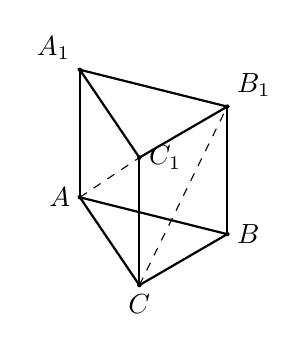
\begin{tikzpicture}[>=stealth,scale=0.72]
  \coordinate (A) at (0,0);
  \coordinate (B) at (2.6,-0.65);
  \coordinate (C) at (1.05,-1.55);
  \coordinate (Aone) at (0,2.25);
  \coordinate (Bone) at (2.6,1.60);
  \coordinate (Cone) at (1.05,0.70);
  \draw[thick] (A)--(B)--(C)--cycle;
  \draw[thick] (Aone)--(Bone)--(Cone)--cycle;
  \draw[thick] (A)--(Aone) (B)--(Bone) (C)--(Cone);
  \draw[dashed] (A)--(Cone) (C)--(Bone);
  \fill (A) circle (1.1pt) node[left] {$A$};
  \fill (B) circle (1.1pt) node[right] {$B$};
  \fill (C) circle (1.1pt) node[below] {$C$};
  \fill (Aone) circle (1.1pt) node[above left] {$A_1$};
  \fill (Bone) circle (1.1pt) node[above right] {$B_1$};
  \fill (Cone) circle (1.1pt) node[right] {$C_1$};
\end{tikzpicture}
\end{center}
\nopagebreak[4]
（1） 建立适当的坐标系，并写出点 $A\text{、}B\text{、}A_1\text{、}C_1$ 的坐标；

（2） 求 $AC_1$ 与侧面 $ABB_1A_1$ 所成的角。

【乙】如图，正方形 $ABCD\text{、}ABEF$ 的边长都是 1，而且平面 $ABCD\text{、}ABEF$ 互相垂直。点 $M$ 在 $AC$ 上移动，点 $N$ 在 $BF$ 上移动，若 $CM=BN=a$（$0<a<\sqrt2$）。
\nopagebreak[4]
\begin{center}% 2002 年全国新课程理科第 18 题乙：两个互相垂直的正方形
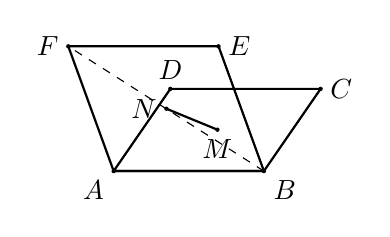
\begin{tikzpicture}[>=stealth,scale=0.72]
  \coordinate (A) at (0,0);
  \coordinate (B) at (2.65,0);
  \coordinate (C) at (3.65,1.45);
  \coordinate (D) at (1.0,1.45);
  \coordinate (E) at (1.85,2.20);
  \coordinate (F) at (-0.80,2.20);
  \coordinate (M) at (1.83,0.73);
  \coordinate (N) at (0.93,1.10);
  \draw[thick] (A)--(B)--(C)--(D)--cycle;
  \draw[thick] (A)--(B)--(E)--(F)--cycle;
  \draw[dashed] (A)--(D) (B)--(F);
  \draw[thick] (M)--(N);
  \fill (A) circle (1.1pt) node[below left] {$A$};
  \fill (B) circle (1.1pt) node[below right] {$B$};
  \fill (C) circle (1.1pt) node[right] {$C$};
  \fill (D) circle (1.1pt) node[above] {$D$};
  \fill (E) circle (1.1pt) node[right] {$E$};
  \fill (F) circle (1.1pt) node[left] {$F$};
  \fill (M) circle (1.1pt) node[below] {$M$};
  \fill (N) circle (1.1pt) node[left] {$N$};
\end{tikzpicture}
\end{center}
\nopagebreak[4]
（1） 求 $MN$ 的长；

（2） $a$ 为何值时，$MN$ 的长最小；

（3） 当 $MN$ 的长最小时，求面 $MNA$ 与面 $MNB$ 所成二面角 $\alpha$ 的大小。

\Needspace{10\baselineskip}
\textbf{解析}

\textbf{甲}

\gksubpart{(1)}

\Needspace{5\baselineskip}
取 $A=(0,0,0)$、$B=(a,0,0)$，令正三角形 $ABC$ 位于 $xOy$ 平面，侧棱方向为 $z$ 轴，则

\nopagebreak[4]
\[
C=\left(\frac a2,\frac{\sqrt3a}{2},0\right),\quad
A_1=(0,0,\sqrt2a),\quad
C_1=\left(\frac a2,\frac{\sqrt3a}{2},\sqrt2a\right).
\]

\gksubpart{(2)}

\Needspace{5\baselineskip}
平面 $ABB_1A_1$ 为 $y=0$，且

\nopagebreak[4]
\[
\overrightarrow{AC_1}
=\left(\frac a2,\frac{\sqrt3a}{2},\sqrt2a\right),\qquad
|\overrightarrow{AC_1}|=\sqrt3a.
\]

\Needspace{5\baselineskip}
若直线与该平面所成角为 $\theta$，则

\nopagebreak[4]
\[
\sin\theta=\frac{\sqrt3a/2}{\sqrt3a}=\frac12,
\]

所以 $\theta=\dfrac\pi6$。

\textbf{乙}

\gksubpart{(1)}

\Needspace{5\baselineskip}
取

\nopagebreak[4]
\[
A=(0,0,0),\quad B=(1,0,0),\quad C=(1,1,0),\quad D=(0,1,0),
\]

\Needspace{5\baselineskip}
以及 $E=(1,0,1)$、$F=(0,0,1)$。令 $t=a/\sqrt2$，则

\nopagebreak[4]
\[
M=(1-t,1-t,0),\qquad N=(1-t,0,t).
\]

\Needspace{5\baselineskip}
因此

\nopagebreak[4]
\[
MN^2=(1-t)^2+t^2=a^2-\sqrt2a+1,
\]

即 $MN=\sqrt{a^2-\sqrt2a+1}$。

\gksubpart{(2)}

\nopagebreak[4]
\[
MN^2=\left(a-\frac{\sqrt2}{2}\right)^2+\frac12,
\]

所以当 $a=\dfrac{\sqrt2}{2}$ 时，$MN$ 最小。

\gksubpart{(3)}

\Needspace{5\baselineskip}
最小值处 $M=(1/2,1/2,0)$、$N=(1/2,0,1/2)$。此时 $\triangle AMN$、$\triangle BMN$ 均为正三角形。设 $H$ 为 $MN$ 的中点，则 $\angle AHB$ 是所求二面角的平面角。计算得

\nopagebreak[4]
\[
\overrightarrow{HA}=\left(-\frac12,-\frac14,-\frac14\right),\qquad
\overrightarrow{HB}=\left(\frac12,-\frac14,-\frac14\right),
\]

\Needspace{5\baselineskip}
且两向量的内积为 $-1/8$，长度平方均为 $3/8$，所以

\nopagebreak[4]
\[
\cos\angle AHB=-\frac13.
\]

\gkanswer{答案（1）：甲：坐标见解析版；乙：$MN=\sqrt{a^2-\sqrt2a+1}$。}

\gkanswer{答案（2）：甲：$\dfrac\pi6$；乙：$a=\dfrac{\sqrt2}{2}$。}

\gkanswer{答案（3）：甲：无此小问；乙：$\alpha=\arccos\left(-\dfrac13\right)$。}

\end{answer}
\begin{answer}
\gksolhead{19}{}

\textbf{题目}：

某单位 6 个员工借助互联网开展工作，每个员工上网的概率都是 0.5（相互独立）。

（1） 求至少 3 人同时上网的概率；

（2） 至少几人同时上网的概率小于 0.3？

\Needspace{4\baselineskip}
\textbf{解析}

设上网人数为 $X$，则 $X\sim B(6,0.5)$。

\gksubpart{(1)}

\nopagebreak[4]
\[
P(X\geqslant3)
=\frac{\binom63+\binom64+\binom65+\binom66}{2^6}
=\frac{21}{32}.
\]

\gksubpart{(2)}

\nopagebreak[4]
\[
P(X\geqslant4)=\frac{22}{64}>0.3,\qquad
P(X\geqslant5)=\frac7{64}<0.3.
\]

因此所求人数为 5。

\gkanswer{答案（1）：$\dfrac{21}{32}$。}

\gkanswer{答案（2）：5 人。}

\end{answer}
\begin{answer}
\gksolhead{20}{}

\textbf{题目}：

\Needspace{5\baselineskip}
已知 $a>0$，函数

\nopagebreak[4]
\[
f(x)=\frac{1-ax}{x},\qquad x\in(0,+\infty).
\]

设 $0<x_1<\dfrac2a$，记曲线 $y=f(x)$ 在点 $M(x_1,f(x_1))$ 处的切线为 $l$。

（1） 求 $l$ 的方程；

（2） 设 $l$ 与 $x$ 轴交点为 $(x_2,0)$。证明：

① $0<x_2\leqslant\dfrac1a$；

② 若 $x_1<\dfrac1a$，则 $x_1<x_2<\dfrac1a$。

\Needspace{4\baselineskip}
\textbf{解析}

\gksubpart{(1)}

\Needspace{5\baselineskip}
将函数写成 $f(x)=1/x-a$，故 $f'(x)=-1/x^2$。在 $x=x_1$ 处的切线为

\nopagebreak[4]
\[
y-\left(\frac1{x_1}-a\right)
=-\frac1{x_1^2}(x-x_1),
\]

\Needspace{5\baselineskip}
即

\nopagebreak[4]
\[
y=-\frac{x}{x_1^2}+\frac2{x_1}-a.
\]

\gksubpart{(2)}

\Needspace{5\baselineskip}
令 $y=0$，得到

\nopagebreak[4]
\[
x_2=2x_1-ax_1^2=x_1(2-ax_1).
\]

\Needspace{5\baselineskip}
由于 $0<x_1<2/a$，有 $x_2>0$。此外

\nopagebreak[4]
\[
\frac1a-x_2
=\frac{(1-ax_1)^2}{a}\geqslant0,
\]

\Needspace{5\baselineskip}
故 $x_2\leqslant1/a$。当 $x_1<1/a$ 时，

\nopagebreak[4]
\[
x_2-x_1=x_1(1-ax_1)>0,
\]

并且上式严格给出 $x_2<1/a$，所以 $x_1<x_2<1/a$。

\gkanswer{答案（1）：$l:y=-\dfrac{x}{x_1^2}+\dfrac2{x_1}-a$。}

\gkanswer{答案（2）：$x_2=2x_1-ax_1^2$；$0<x_2\leqslant\dfrac1a$，且当 $x_1<\dfrac1a$ 时 $x_1<x_2<\dfrac1a$。}

\end{answer}
\begin{answer}
\gksolhead{21}{}

\textbf{题目}：

已知两点 $M(-1,0)\text{、}N(1,0)$，且点 $P$ 使 $\overrightarrow{MP}\cdot\overrightarrow{MN}$、$\overrightarrow{PM}\cdot\overrightarrow{PN}$、$\overrightarrow{NM}\cdot\overrightarrow{NP}$ 成公差小于零的等差数列。

（1） 点 $P$ 的轨迹是什么曲线？

（2） 若点 $P$ 坐标为 $(x_0,y_0)$，记 $\theta$ 为 $\overrightarrow{PM}$ 与 $\overrightarrow{PN}$ 的夹角，求 $\tan\theta$。

\Needspace{4\baselineskip}
\textbf{解析}

\gksubpart{(1)}

\Needspace{5\baselineskip}
设 $P=(x,y)$。三个数量分别为

\nopagebreak[4]
\[
u=\overrightarrow{MP}\cdot\overrightarrow{MN}=2(x+1),
\]

\nopagebreak[4]
\[
v=\overrightarrow{PM}\cdot\overrightarrow{PN}=x^2+y^2-1,
\]

\nopagebreak[4]
\[
w=\overrightarrow{NM}\cdot\overrightarrow{NP}=2(1-x).
\]

\Needspace{5\baselineskip}
等差条件给出 $u+w=2v$，于是

\nopagebreak[4]
\[
x^2+y^2=3.
\]

公差为 $w-v=-2x$，其小于零等价于 $x>0$。故轨迹是圆 $x^2+y^2=3$ 的右半圆。

\gksubpart{(2)}

\Needspace{5\baselineskip}
在轨迹上 $v=2$，而 $\overrightarrow{PM}$ 与 $\overrightarrow{PN}$ 的叉积绝对值为 $2|y|$，所以

\nopagebreak[4]
\[
\tan\theta=\frac{2|y_0|}{2}=|y_0|.
\]

\gkanswer{答案（1）：圆 $x^2+y^2=3$ 的右半圆（$x>0$）。}

\gkanswer{答案（2）：$\tan\theta=|y_0|$。}

\end{answer}
\begin{answer}
\gksolhead{22}{}

\textbf{题目}：

\Needspace{5\baselineskip}
已知 $\{a_n\}$ 是由非负整数组成的数列，满足 $a_1=0\text{、}a_2=3$，

\nopagebreak[4]
\[
a_{n+1}a_n=(a_{n-1}+2)(a_{n-2}+2),\qquad n=3,4,5,\cdots.
\]

（1） 求 $a_3$；

（2） 证明 $a_n=a_{n-2}+2$，$n=3,4,5,\cdots$；

（3） 求 $\{a_n\}$ 的通项公式及其前 $n$ 项和 $S_n$。

\Needspace{4\baselineskip}
\textbf{解析}

\gksubpart{(1)}

\Needspace{5\baselineskip}
由 $n=3$ 得

\nopagebreak[4]
\[
a_4a_3=(a_2+2)(a_1+2)=10.
\]

\Needspace{5\baselineskip}
因此 $a_3$ 是 $10$ 的正因数。再由 $n=4$，

\nopagebreak[4]
\[
a_5a_4=(a_3+2)(a_2+2)=5(a_3+2),
\]

\Needspace{5\baselineskip}
结合 $a_4=10/a_3$ 得

\nopagebreak[4]
\[
a_5=\frac{a_3(a_3+2)}2.
\]

\Needspace{5\baselineskip}
由非负整数条件，$a_3=1\text{、}5$ 时 $a_5$ 不是整数，只剩 $a_3=2\text{、}10$。若 $a_3=10$，则 $a_4=1\text{、}a_5=60$，由 $n=5$ 得

\nopagebreak[4]
\[
a_6a_5=(a_4+2)(a_3+2)=36,
\]

这会使 $a_6=3/5$，矛盾。因此 $a_3=2$。

\gksubpart{(2)}

\Needspace{5\baselineskip}
由上面的计算还得到 $a_4=5$，故

\nopagebreak[4]
\[
a_3=a_1+2,\qquad a_4=a_2+2.
\]

\Needspace{5\baselineskip}
若对某个 $k\geqslant3$ 有 $a_k=a_{k-2}+2$，则递推式给出

\nopagebreak[4]
\[
a_{k+1}a_k=(a_{k-1}+2)(a_{k-2}+2)
=(a_{k-1}+2)a_k.
\]

因 $a_k>0$，可约去 $a_k$，得到 $a_{k+1}=a_{k-1}+2$。由归纳法，$a_n=a_{n-2}+2$ 对所有 $n\geqslant3$ 成立。

\gksubpart{(3)}

\Needspace{5\baselineskip}
奇数项和偶数项分别为

\nopagebreak[4]
\[
a_{2k-1}=2k-2,\qquad a_{2k}=2k+1,
\]

\Needspace{5\baselineskip}
统一写为

\nopagebreak[4]
\[
a_n=n+(-1)^n.
\]

\Needspace{5\baselineskip}
因此

\nopagebreak[4]
\[
S_n=\sum_{k=1}^n\bigl(k+(-1)^k\bigr)
=\frac{n(n+1)}2+\frac{(-1)^n-1}{2}.
\]

\gkanswer{答案（1）：$a_3=2$。}

\gkanswer{答案（2）：$a_n=a_{n-2}+2$，$n=3,4,5,\cdots$。}

\gkanswer{答案（3）：$a_n=n+(-1)^n$；$S_n=\dfrac{n(n+1)}2+\dfrac{(-1)^n-1}{2}$。}

\end{answer}
